\documentclass{article}
\usepackage[utf8]{inputenc}
\usepackage{graphicx}
\renewcommand{\figurename}{Gambar 3.}
\renewcommand*\contentsname{Daftar Isi}
\renewcommand*\abstractname{Abstrak}

\title{PEMBUATAN PERANGKAT LUNAK PENJUALAN BARANG ELEKTRONIK}
\author{ ARI CHANDRA HINTA }
\date{Desember 2019}
\graphicspath{{Images/}}

\begin{document}

\maketitle

\begin{abstract}


Perkembangan teknologi informasi di Indonesia telah banyak mengalami kemajuan. Hal ini juga diikuti dengan perkembangan bisnis penjualan. Perkembangan bisnis penjualan tersebut berdampak langsung pada peningkatan arus transaksi yang dilakukan perusahaan. Kecepatan dalam pelayanan menjadi salah satu kebutuhan utama untuk mencapai tujuan perusahaan.

Aplikasi penjualan merupakan salah satu pilihan yang diharapan dapat membantu proses transaksi penjualan secara tunai. Aplikasi penjualan ini dapat digunakan oleh usaha retail khususnya barang elektronik.

Keunggulan aplikasi ini memiliki tampilan yang user friendly dan mudah digunakan, handal dalam menangani transaksi dan biaya pengadaannya tidak terlalu mahal karena tidak menuntut spesifikasi komputer yang terlalu tinggi.


\end{abstract}
\newpage
\tableofcontents
\newpage
\section{Pendahuluan}
\subsection{Latar Belakang Masalah}
Perkembangan teknologi informasi di Indonesia telah banyak mengalami kemajuan. hal ini juga diikuti dengan perkembangan bisnis penjualan. Perkembangan bisnis penjualan tersebut berdampak langsung pada peningkatan arus transaksi yang dilakukan perusahaan. Kecepatan dalam pelayanan menjadi salah satu kebutuhan utama untuk mencapai tujuan perusahaan.

Mengingat arus transaksi yang semakin padat, sedangkan kecepatan dalam pelayanan adalah faktor yang utama, maka pencatatan transaksi secara manual tentu kurang dapat diandalkan. Kendala yang dihadapi dengan menggunakan pencatatan transaksi secara manual, yang pertama adalah waktu. Pencatatan transaksi secara manual membutuhkan waktu yang lama. Sedangkan yang kedua adalah tingkat akurasi atau ketelitian. Tidak dapat dipungkiri, pencatatan transaksi secara manual rentan terhadap human error atau kesalahan manusia. Dan untuk mengatasinya, perusahaan biasanya membuat suatu cara kerja atau model pencatatan tertentu.

Oleh karena itu, dibutuhkan suatu perangkat lunak yang menggantikan pencatatan transaksi secara manual. Perangkat lunak tersebut diharapkan dapat lebih menyingkat waktu dibandingkan pencatatan transaksi secara manual. Di samping itu, perangkat lunak penjualan ini juga diharapkan meningkatkan ketelitian dan meminimalisasi human error atau kesalahan manusia.

Berdasarkan uraian di atas penulis mengambil judul “PEMBUATAN PERANGKAT LUNAK PENJUALAN BARANG ELEKTRONIK”.

\subsection{Identifikasi dan Batasan Masalah}
Penulis mengidetifikasikan masalah yang ada adalah sebagai berikut :

Bagaimana membuat perangkat lunak yang menangani penjualan barang elektronik?

Hal – hal yang menjadi batasan dalam penelitian yang akan dikemukakan oleh penulis adalah sebagai berikut :
\begin{enumerate}
    \item Hanya menguraikan transaksi – transaksi penjualan barang elektronik rumah tangga secara tunai.
    \item Program ini dibuat hanya sebagai aplikasi stand alone, bukan jaringan.
    \item Informasi yang dihasilkan hanya berupa laporan penjualan dan daftar barang.
\end{enumerate}
\subsection{Maksud dan Tujuan}
Maksud dari pembuatan perangkat lunak ini adalah agar berguna dalam segi bisnis dan pengembangan ilmu komputer.

Tujuan dari pembuatan program ini adalah menciptakan suatu solusi yang dapat memudahkan pencatatan transaksi penjualan yang terkomputerisasi.

\subsection{Kegunaan}
Adapun kegunaan penelitian yang dilakukan oleh penulis adalah sebagai berikut:

\begin{enumerate}
    \item Di Bidang keilmuan \newline
    Penulis dapat memperdalam penguasaan Microsoft Access yang telah didapat di bangku kuliah.
   
    \item Bagi peneliti/programmer selanjutnya \newline
    Peneliti lain dapat menjadikan hasil perancangan yang penulis lakukan sebagai bahan referensi atau mengembangkan judul yang relevan.
    
    \item Di bidang praktisi \newline
    Hasil penelitian yang penulis lakukan dapat memberikan alternatif bagi perusahaan retail untuk memperbaiki pencatatan yang manual menjadi terkomputerisasi.
\end{enumerate}

\subsection{Metode Pendekatan}
Metode yang digunakan

\begin{enumerate}
    \item Metode Penelitian \newline
    Dalam penelitian yang penulis lakukan ini, penulis menggunakan metode deskriptif, yaitu dengan memaparkan/menjelaskan secara jelas dan sistematis mengenai langkah-langkah perancangan perangkat lunak.
    \item Teknik Pengumpulan Data \newline
    Teknik pengumpulan data yaitu dengan studi pustaka, mempelajari dan menelaah buku – buku yang menunjang dengan judul yang penulis ambil. Adapun buku – buku dipelajari oleh penulis yaitu yang tercantum di dalam daftar pustaka.
\end{enumerate}
\subsection{Sistematika Penulisan}
Untuk memberikan gambaran isi laporan ini, penulis akan menguraikan susunan laporan secara garis besar yang terdiri dari lima bab, dimana setiap babnya akan dibagi menjadi beberapa sub bab. Sistematika penulisan ini dibuat tersusun dengan tujuan agar mudah dipahami oleh semua pihak. Adapun susunannya sebagai berikut :

\begin{enumerate}
    \item BAB I 	PENDAHULUAN \newline
    Pendahuluan berisi tentang latar belakang, identifikasi masalah yang dihadapi, batasan masalah, maksud dan tujuan pembuatan aplikasi, kegunaan pembuatan aplikasi, dan sistematika penulisan
    \item BAB II	TINJAUAN PUSTAKA \newline
    Bab ini berisi landasan teori yang relevan dengan judul dan faktor-faktor dasar yang mendukung penyelesaian masalah.
    \item BAB III	CARA KERJA PERANGKAT LUNAK \newline
    Pada bab ini memaparkan tentang  cara kerja perangkat lunak transaksi penjualan barang elektronik.
    \item BAB IV	IMPLEMENTASI \newline
    Pada bab ini berisi pembuatan perangkat lunak  penjualan, kode-kode program, perancangan form dan laporan yang terlibat.
    \item BAB V	KESIMPULAN DAN SARAN \newline
    Dalam bab ini penulis menyimpulkan mengenai pembuatan perangkat lunak yang telah dilakukan serta memberikan saran yang mungkin dijadikan sebagai bahan pertimbangan.
\end{enumerate}

\section{Tinjauan Pustaka}
\subsection{Pengertian Perangkat Lunak}
Menurut Rono Satria Wahono, perangkat lunak dapat didefinisikan : “Suatu program yang berisikan instruksi untuk melakukan pengolahan  data” (Internet dan Web Server, 2004, hal.12).

Perangkat lunak digolongkan menjadi beberapa jenis, yaitu

\begin{enumerate}
    \item Sistem Operasi \newline
    Adalah software yang berfungsi untuk mengaktifkan seluruh perangkat yang terpasang pada komputer sehingga masing-masingnya dapat saling berkomunikasi. Tanpa ada sistem operasi maka komputer tak dapat difungsikan sama sekali. Contohnya sistem operasi adalah  DOS, Unix, Novell, OS/2, Windows.
    \item Program Utility \newline
    Program utility berfungsi untuk membantu atau mengisi kekurangan/ kelemahan dari sistem operasi, misalnya PC Tools dapat melakukan perintah format sebagaimana DOS, tapi PC Tools mampu memberikan keterangan dan animasi yang bagus dalam proses pemformatan. File yang telah dihapus oleh DOS tidak dapat dikembalikan lagi tapi dengan program bantu hal ini dapat dilakukan. Contoh program utility adalah Norton Utility, Scandisk, PC Tools.
    \item Program Aplikasi \newline
    Merupakan program yang khusus melakukan suatu pekerjaan tertentu, seperti program gaji pada suatu perusahaan. Maka program ini hanya digunakan oleh bagian keuangan saja tidak dapat digunakan oleh departemen yang lain. Biasanya program aplikasi ini dibuat oleh seorang programmer komputer sesuai dengan permintaan/kebutuhan seseorang/ lembaga/ perusahaan guna keperluan interennya. Contohnya  seperti GL, MYOB, Payroll, dan aplikasi penjualan.
    \item Program Paket \newline
    Adalah program yang disusun sedemikian rupa sehingga dapat digunakan oleh banyak orang dengan berbagai kepentingan. Seperti MS-Word, dapat digunakan oleh departemen keuangan untuk membuat nota, atau bagian administrasi untuk membuat surat penawaran dan lain sebagainya. Contohnya seperti MS-Word, MS-Excel, Lotus 125.
    
    \item Bahasa Pemograman
    , Pascal, Fortran, Clipper, dBase, dll. Merupakan software yang khusus digunakan untuk membuat program komputer, apakah itu sistem operasi, atau program paket. Bahasa pemrograman ini biasanya dibagi atas 3 tingkatan, yaitu 
    \begin{enumerate}
        \item Low Level Language, bahasa pemrograman generasi pertama, bahasa pemrograman jenis ini sangat sulit dimengerti karena instruksinya menggunakan bahasa mesin. 
        \item Midle Level Language, merupakan bahasa pemrograman tingkat menengah dimana penggunaan instruksi sudah mendekati bahasa sehari-hari, walaupun begitu masih sulit untuk dimengerti karena banyak menggunakan singkatan-singakatan seperti STO artinya simpan (singkatan dari STORE) dan MOV artinya pindah (singkatan dari MOVE).Yang tergolong kedalam bahasa ini adalah Assembler, ForTran (Formula Translator).
        \item High Level Language, merupakan bahasa tingkat tinggi yang mempunyai ciri mudah dimengerti, karena menggunakan bahasa sehari-hari, seperti BASIC, COBOL, dBase.
    \end{enumerate}
\end{enumerate}

\subsection{Pengertian Penjualan}
Menurut Zaki Baridwan, penjualan dapat didefinisikan : “Penjualan adalah kegiatan penukaran produk atau jasa yang ditawarkan perusahaan kepada konsumen dengan sejumlah nominal yang ditetapkan, dan prosesnya dapat dilakukan secara tunai ataupun kredit.” (Prosedur dan Metode Penyusunan Sistem Akuntansi,1981,hal 5).

Disini pembahasan penjualan dibatasi pada penjualan secara tunai. Transaksi penjualan secara umum melibatkan beberapa komponen seperti tanggal transaksi, no nota, nama barang, harga per unit, jumlah pembelian dan total harga. Pencatatan merupakan unsur yang penting, yaitu sebagai bukti tertulis dari transaksi yang dilakukan Kendala yang sering ditemui dalam pencatatan transaksi penjualan secara manual diantaranya,
\begin{enumerate}
    \item Prosesnya lama dan panjang.
    \item Sering terjadi kesalahan pencatatan.
    \item Pencatatan adalah bukti tertulis dari transaksi yang dilakukan, karena itu sebaiknya dibuat dengan rapi. Pencatatan manual umumnya tidak sebaik cetakan printer.
    \item Pada praktiknya.Pencatatan manual memungkinkan terjadi kecurangan pada praktiknya.
\end{enumerate}
\subsection{Pengertian Perangkat Lunak Penjualan}
Perangkat lunak penjualan merupakan program yang dibuat khusus untuk menangani transaksi penjualan, dan disesuaikan dengan kebutuhan internnya.. Maka program ini hanya digunakan oleh untuk penjualan saja, dan tidak dapat digunakan untuk kebutuhan diluar itu.

Perangkat lunak penjualan ini adalah suatu proses terkomputerisasi atau berbasis komputer. proses yang terkomputerisasi memiliki banyak kelebihan dibandingkan proses manual. Komputerisasi dilakukan oleh suatu instansi jika alasan-alasan dibawah ini terpenuhi, yaitu.
\begin{enumerate}
    \item Proses tanpa komputerisasi memerlukan proses lama dan panjang.
    \item Proses tanpa komputerisasi membutuhkan sumber daya yang sebenarnya dapat dihilangkan oleh komputerisasi.
    \item Proses tanpa komputerisasi membutuhkan biaya yang besar.
    \item Proses tanpa komputerisasi tertinggal dengan pesaing bisnis dalam segi inovasi teknologi.
    \item Proses tanpa komputerisasi terdapat masalah, misalnya memungkinkan terjadi kecurangan.
\end{enumerate}

Tidak semua proses tanpa komputerisasi buruk, oleh karena itu instansi yang ingin menerapkan komputerisasi harus merencanakan dan mempertimbangkan dengan seksama faktor-faktor berikut ini
\begin{enumerate}
    \item Biaya investasi awal.
    \item Biaya perawatan.
    \item Jumlah sumber daya manusia yang dibutuhkan.
    \item Kemudahan komputerisasi.
    \item Keuntungan yang diraih.
    \item Kemudahan pengembangan teknologi.
\end{enumerate}

\subsection{Barang Elektronik}
Barang elektronik adalah barang yang membutuhkan sumber daya listrik sebagai penggeraknya. Barang elektronik dewasa ini sudah banyak sekali digunakan dalam kehidupan sehari-hari, dan dapat dikelompokkan menjadi :
\begin{enumerate}
    \item Barang elektronik rumah tangga \newline
    Yaitu barang elektronik yang fungsinya sebagai pembantu pekerjaan rumah tangga. Contohnya
    \begin{enumerate}
        \item Kompor gas
        \item Mesin cuci
        \item Blender, rice cooker dan sejenisnya
    \end{enumerate}
    \item Barang elektronik hiburan \newline
     Yaitu barang elektronik yang fungsinya sebagai hiburan,misalnya
    \begin{enumerate}
        \item Televisi dan radio
        \item VCD Player, MP3 Player, speaker dan sejenisnya.
\end{enumerate}
    \item Barang elektronik penunjang pekerjaaan \newline Barang elektronik jenis ini agak berbeda dengan elektronik rumah tangga karena digunakan untuk menunjang kegiatan di lingkungan kerja yang lebih spesifik seperti di kantor, sekolah dan sebagainya dan untuk mengoperasikannya biasanya membutuhkan keahlian. Contohnya
    \begin{enumerate}
        \item Komputer
        \item Mesin tik elektronik
        \item Proyektor, printer, dan sejenisnya.
    \end{enumerate}
    \item Barang elektronik untuk komunikasi \newline
    Fungsinya lebih spesifik, yaitu untuk keperluan komunikasi. Contohnya telepon, faximile dan sejenisnya.
\end{enumerate}

Perkembangan barang elektronik tergolong pesat, dan masih banyak jenis-jenis barang-barang elektronik lainnya yang dibuat untuk tujuan spesifik Barang elektronik yang dibahas dalam aplikasi penjualan ini adalah barang elektronik rumah tangga.

\section{Cara Kerja Perangkat Lunak}
\subsection{Gambaran Umum}
Perangkat lunak penjualan yang akan dibuat mengikuti prinsip sederhana penjualan, yaitu penjualan akan mengurangi stok barang. Untuk menambah stok dan jenis barang, ditambahkan juga form pembelian barang, sehingga aplikasi ini juga dapat menangani transaksi pembelian barang.

Berikut ini adalah skema gambaran umum proses input – output dalam aplikasi penjualan

\begin{figure}[htp]
    \centering
    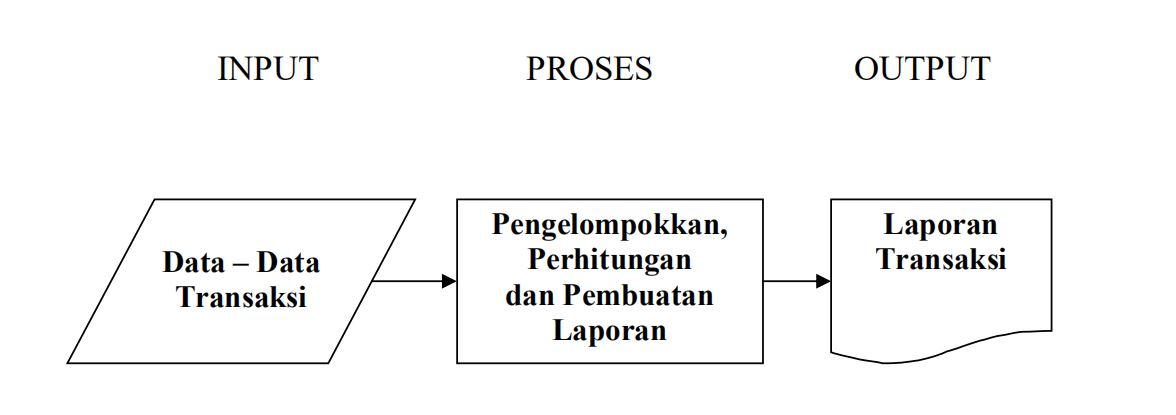
\includegraphics[width=12cm]{gambar_3_1.JPG}
    \caption{ Skema Input – Proses – Output dalam aplikasi penjualan.}
    \label{fig:my_label}
\end{figure}

\subsubsection{Proses Input}
Yaitu proses memasukkan data ke dalam program dan biasanya proses ini dilakukan oleh operator (misalnya pramuniaga). Data-data yang dimasukkan pada proses ini antara lain
\begin{enumerate}
    \item Data Transaksi Penjualan \newline
    Sebagian besar data ini didapat dari konsumen, misalnya nama konsumen dan data barang yang dibeli.
    \item Data Retur \newline
    Data retur adalah data barang yang dikembalikan oleh pelanggan.
    \item Data Barang \newline
    Data barang berupa kode, nama, dan harga barang dan keterangan lain yang diperlukan.
    \item Data Pelanggan \newline
    Yaitu data konsumen perorangan/instansi yang menjadi pelanggan. Dalam transaksi penjualan akan lebih mempermudah pencatatan jika konsumen terdaftar sebagai pelanggan, sehingga tidak perlu lagi mengetik ulang data konsumen.
\end{enumerate}
\subsubsection{Proses Pengelompokan, Perhitungan dan Pembuatan Laporan}
Proses ini dilakukan oleh operator program dan otomatisasi program sendiri. Penjelasan proses ini adalah sebagai berikut 
\begin{enumerate}
    \item Proses Pengelompokkan.\newline
    Operator program mengelompokkan transaksi dan membuka form yang tepat, misalnya untuk transaksi penjualan operator akan membuka form penjualan.
    \item Proses Penghitungan\newline
    Proses ini dilakukan oleh program, misalnya saat operator mengisi form penjualan barang maka harga barang akan dihitung dan ditampilkan secara otomatis. Begitu juga dengan stok barang akan langsung dikurangi sesuai jumlah pembelian, dan itu dilakukan secara otomatis pula.
    \item Pembuatan Laporan \newline
    Operator memilih laporan apa yang akan dicetak, dan program akan langsung mencetak sesuai dengan yang diminta oleh operator.
\end{enumerate}

\subsubsection{Cara Kerja Perangkat Lunak}
Cara kerja perangkat lunak penjualan ini adalah
\begin{enumerate}
    \item Operator memasukkan data-data transaksi yang dilakukan
    \item Program menerima data-data tersebut dan melakukan proses sesuai dengan data-data transaksi yang diterima
    \item Program mencetak laporan yang dibutuhkan sesuai permintaan operator program.
\end{enumerate}

\subsubsection{Transaksi yang ditangani Perangkat Lunak}
Perangkat lunak penjualan diprogram untuk menangani transaksi sebagai berikut:

\begin{enumerate}
    \item Transaksi Penjualan Barang \newline 
    Desain form penjualan dibuat lengkap dan mudah, sehingga operator program dapat mencatat data-data transaksi yang diperlukan dengan lengkap dan cepat. Total pembayaran juga langsung dihitung otomatis oleh program dan operator dapat langsung mencetak notanya. Program juga secara otomatis akan langsung mengurangi jumlah stok sesuai dengan penjualan.
    \item Transaksi Retur Penjualan \newline 
    Transaksi retur berarti pengembalian barang karena kondisi barang tidak sesuai dengan perjanjian. Dengan demikian, maka retur penjualan adalah pengembalian barang oleh konsumen karena kondisi barang cacat atau tidak sesuai perjanjian. Retur penjualan diproses oleh program berupa pembatalan, pengurangan atau perubahan jumlah stok akibat transaksi penjualan yang sebelumnya dilakukan.
\end{enumerate}

\subsubsection{Laporan yang dihasilkan}
Program penjualan ini dapat mencetak informasi berupa laporan sebagai berikut
\begin{enumerate}
    \item Laporan Transaksi Penjualan \newline
    Agar menghasilkan informasi yang aktual dan sesuai kebutuhan, laporan transaksi penjualan dapat dicetak berdasarkan
    \begin{enumerate}
        \item Nomor Transaksi
        \item Tanggal transaksi
        \item Kode pelanggan
    \end{enumerate}
    Format kedua laporan dapat dipilih dalam dua tampilan, yaitu
    \begin{enumerate}
        \item Tampilan ringkas (summary). \newline
        Menyajikan laporan transaksi hanya jumlah keseluruhan.
        \item Tampilan detail \newline
        Menyajikan laporan transaksi secara lengkap, dan menyertakan  data item barang setiap transaksi yang dicatat.
    \end{enumerate}
    \item Faktur penjualan \newline
    Faktur ini dicetak dan diberikan kepada konsumen dan dicetak setelah transaksi selesai dilakukan.
    \item Daftar Barang \newline
    Daftar barang dapat dicetak berdasarkan :
    \begin{enumerate}
        \item Kode barang
        \item Tipe barang
    \end{enumerate}
\end{enumerate}
\newpage
\subsection{Rancangan Tampilan Form Database}
\subsubsection{Rancangan Form Daftar Barang}
Form ini dirancang untuk memanipulasi (menambah, menghapus,merubah) data barang. Data yang diisikan pada form ini disimpan dalam tabel barang.
    \begin{figure}[htp]
        \centering
        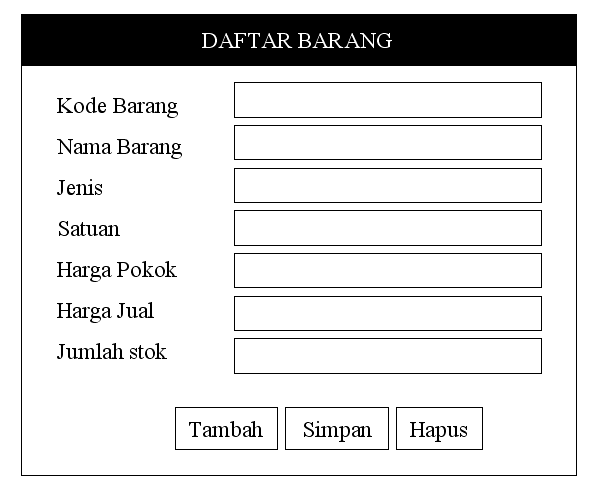
\includegraphics[width=12cm]{gambar_3_2.png}
        \caption{Rancangan form daftar barang}
        \label{fig:my_label2}
    \end{figure}
    \newpage
\subsubsection{Rancangan Form Pelanggan}
Form ini dirancang untuk memanipulasi (menambah, menghapus,merubah) data pelanggan. Data yang diisikan pada form ini disimpan dalam tabel pelanggan.
\begin{figure}[htp]
    \centering
    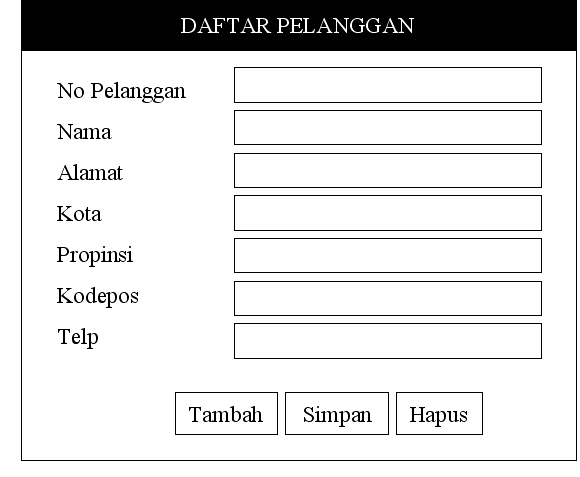
\includegraphics[width=11cm]{gambar_3_3.png}
    \caption{Rancangan form pelanggan}
    \label{fig:my_label3}
\end{figure}

\subsubsection{Rancangan Form Transaksi}
Form ini dirancang untuk menangani transaksi penjualan dan retur (pengembalian). Untuk merubah status transaksi (penjualan atau retur), dapat dipilih dari combobox status.
\begin{figure}[htp]
    \centering
    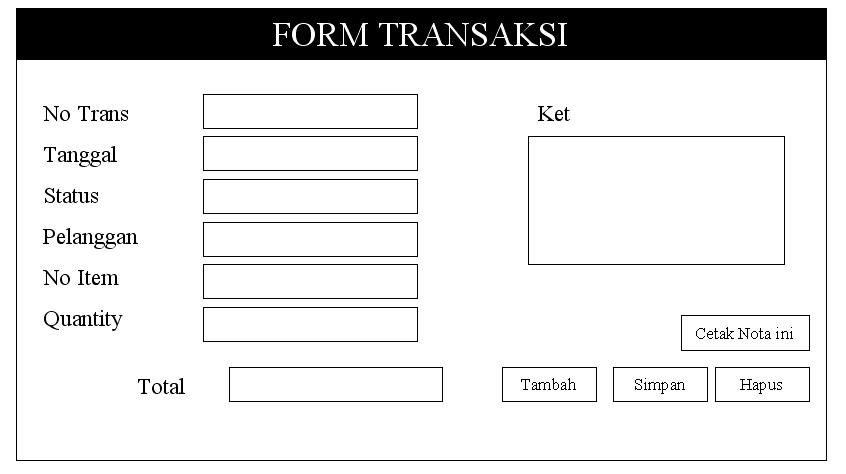
\includegraphics[width=11cm]{gambar_3_4.png}
    \caption{Rancangan form transaksi}
    \label{fig:my_label4}
\end{figure}
\newpage

\subsubsection{Rancangan Form Cetak Transaksi}
Form ini dirancang untuk menyeleksi laporan dan memilih format laporan yang akan dicetak. Form laporan dapat dipilih dua mode, yaitu mode Summary (hanya menampilkan jumlah total transaksinya) atau mode detail (menampilkan seluruh data transaksi secara lengkap).
\begin{figure}[htp]
    \centering
    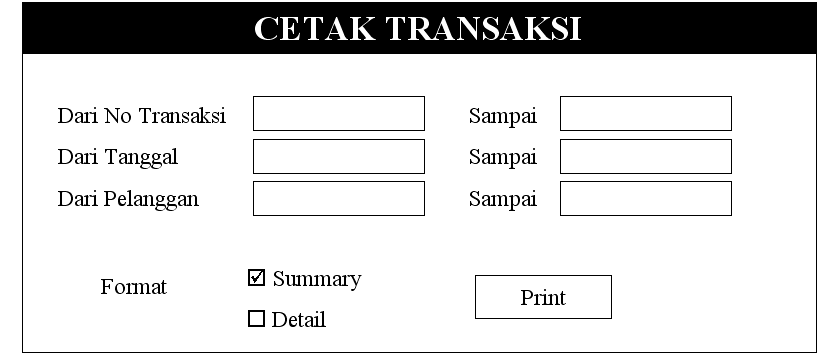
\includegraphics[width=11cm]{gambar_3_5.png}
    \caption{ Rancangan form cetak transaksi.}
    \label{fig:my_label5}
\end{figure}
\subsubsection{Rancangan ERD}
ER diagram menampilkan setiap entitas lengkap dengan atributnya, dan nantinya akan diimplementasikan menjadi sebuah database. Sedangkan setiap entitas akan menjadi tabel.
\begin{figure}[htp]
    \centering
    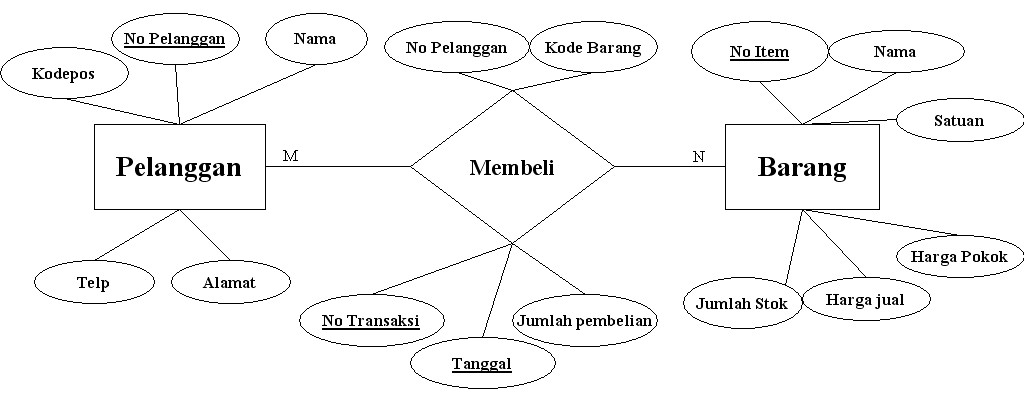
\includegraphics[width=12cm]{gambar_3_6.png}
    \caption{ Pemodelan dengan ER Diagram.}
    \label{fig:my_label6}
\end{figure}
\newpage
Dari gambar diatas, dapat dilihat relasi antara entitas pelanggan dan entitas barang memiliki derajat Many to Many, sehingga himpunan relasinya diimplementasikan menjadi sebuat tabel baru.

\subsubsection{Struktur Tabel}
Struktur tabel dari database aplikasi penjualan adalah sebagai berikut :

\begin{table}[h!]
\centering
\begin{tabular}{||c c c ||} 
 \hline
 Field & Tipe Data & Size \\ [0.5ex] 
 \hline\hline
NoPelanggan & String & 5 \\
Nama & String & 50 \\
Alamat & String & 50 \\
Kota & String & 30 \\
Propinsi & String & 30 \\
Kode Pos & String & 6 \\
Telepon & String & 20 \\ [1ex]
 \hline
\end{tabular}
\caption{Struktur tabel pelanggan.}
\label{table:1}
\end{table}

\begin{table}[h!]
\centering
\begin{tabular}{||c c c ||} 
 \hline
 Field & Tipe Data & Size \\ [0.5ex] 
 \hline\hline
NoItem & String & 5 \\
Jenis Barang & String & 30 \\
Satuan & String & 30 \\
Harga Pokok & Numeric & \\	
Harga jual & Numeric & \\	
Quantity & Numeric & \\
Keterangan & String & 30 \\ [1ex]
 \hline
\end{tabular}
\caption{Struktur tabel barang.}
\label{table:2}
\end{table}

\begin{table}[h!]
\centering
\begin{tabular}{||c c c c ||} 
 \hline
 Field & Tipe Data & Size & Ket \\ [0.5ex] 
 \hline\hline
No Transaksi & String  & 8 & 5 \\
Tanggal & Date & -  & \\	
No Pelanggan & String & 5 & \\	
Total Qty & Numeric & &  \\		
Total Jual & Numeric & & \\		
Status & String & 15 & Penjualan /retur \\
Keterangan & String & 50 & 30 \\ [1ex]
 \hline
\end{tabular}
\caption{Struktur tabel transaksi.}
\label{table:3}
\end{table}

\section{Implementasi}
\subsection{Tahapan - Tahapan}
Implementasi pembuatan perangkat lunak penjualan disusun secara sistematis, mulai dari pembuatan tabel, relasi antar tabel, query, pembuatan form, pembuatan report  sampai dengan pembuatan menu utama sehingga menjadi suatu aplikasi yang utuh.

\subsubsection{Struktur Tabel}
Pada setiap struktur table terdapat field name yang terdiri dari beberapa record dan tipe data untuk memilih tipe apa saja yang akan digunakan dan description untuk mendeskripsikan record.
\begin{enumerate}
    \item Tabel Barang \newline
    Tabel barang terdiri dari 8 field name, yaitu NoItem, Keterangan, JenisItem, Satuan, HargaPokok, hargaJual, QtyStock, Note.
    \begin{table}[h!]
    \centering
    \begin{tabular}{||c c c ||} 
     \hline
     Field & Tipe Data & Size \\ [0.5ex] 
     \hline\hline
    NoItem & Text & 5 \\
    Jenis Barang & Text & 30 \\
    Satuan & Text & 30 \\
    Harga Pokok & Number & Long Integer\\	
    Quantity & Number & Integer\\
    Keterangan & Text & 50 \\ [1ex]
     \hline
    \end{tabular}
    \caption{Tabel item.}
    \label{table:4}
    \end{table}
    \newpage
    \item Tabel Pelanggan \newline
    Tabel pelanggan terdiri dari field-field yang berhubungan dengan data pelanggan.
\begin{table}[h!]
\centering
\begin{tabular}{||c c c ||} 
 \hline
 Field & Tipe Data & Size \\ [0.5ex] 
 \hline\hline
NoPelanggan & Text & 5 \\
Nama & Text & 50 \\
Alamat & Text & 50 \\
Kota & Text & 30 \\
Propinsi & Text & 30 \\
Kode Pos & Text & 6 \\
Telepon & Text & 20 \\ [1ex]
 \hline
\end{tabular}
\caption{Tabel pelanggan.}
\label{table:5}
\end{table}
    \item Tabel Penjualan \newline
    Terdiri dari NoTransaksi, status, tanggal, Nopelanggan, Note, TotalQty dan TotalBeli. 
\begin{table}[h!]
\centering
\begin{tabular}{||c c c c ||} 
 \hline
 Field & Tipe Data & Size & Ket \\ [0.5ex] 
 \hline\hline
No Transaksi & Text  & 8 & \\
Tanggal & Date & -  & \\	
No Pelanggan & Text & 5 & \\	
Total Qty & Number & Integer &  \\		
Total Jual & Number & Long Integer  & \\		
Status & Text & 15 & Penjualan /retur \\
Keterangan & Text & 50 &  \\ [1ex]
 \hline
\end{tabular}
\caption{Tabel penjualan header.}
\label{table:6}
\end{table}
\newpage
    \item Tabel Penjualan Detail \newline
    Tabel pembelian detail terdiri dari field-field pelengkap dari tabel transaksi penjualan. Tabel pembelian detail dipisahkan dari tabel transaksi, karena dengan satu Nomor Transaksi pelanggan bisa membeli banyak item barang.
     \begin{table}[h!]
    \centering
    \begin{tabular}{||c c c ||} 
     \hline
     Field & Tipe Data & Size \\ [0.5ex] 
     \hline\hline
No Transaksi & Text & 8 \\
NoBaris & Number & Integer \\
NoItem & Text & 5 \\ 
Quantity & Number & Integer \\
hargaJual & Number & Long Integer \\
Total & Number & Long Integer \\ [1ex]
     \hline
    \end{tabular}
    \caption{Tabel penjualan detail.}
    \label{table:7}
    \end{table}

    \item Tabel Satuan \newline
    Terdiri dari  field-field sebagai keterangan dari satuan barang. Seperti tabel jenisitem, pada tabel satuan terdapat field default yang bernilai true/false. Fungsinya jika default bernilai true, maka satuan tersebut akan dijadikan pilihan standard dalam pengisian data barang.
    \begin{table}[h!]
    \centering
    \begin{tabular}{||c c c ||} 
     \hline
     Field & Tipe Data & Size \\ [0.5ex] 
     \hline\hline
Satuan & Text & 20\\
Keterangan & Text & 50\\
Default & Text & 20\\ [1ex]
     \hline
    \end{tabular}
    \caption{Tabel satuan.}
    \label{table:8}
    \end{table}
\end{enumerate}
\newpage
\subsubsection{Relasi Antar Tabel}
\renewcommand{\figurename}{Gambar 4.}
Relasi antar tabel dibawah ini menggambarkan field dari suatu tabel memiliki hubungan dengan field dari tabel yang lain, yang dimodelkan dengan garis tebal.
\begin{figure}[htp]
    \centering
    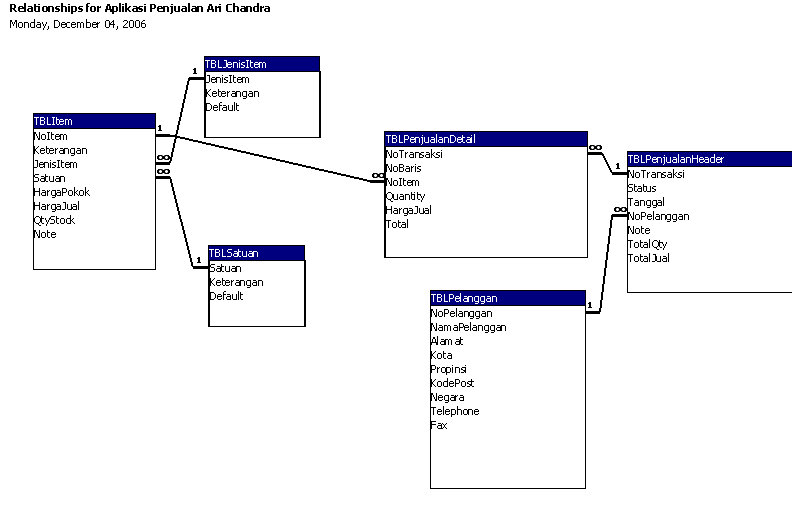
\includegraphics[width=14cm]{gambar_4_1.png}
    \caption{Relasi antar tabel.}
    \label{fig:41}
\end{figure}
\newpage

\subsubsection{Query}
Query adalah fasilitas dalam Microsoft Access yang digunakan untuk mencari dan menampilkan data yang memenuhi syarat tertentu dari satu table atau lebih. Query dapat juga digunakan untuk meng-update atau menghapus beberapa record data pada satu saat yang sama. Selain itu dapat juga melakukan perhitungan terhadap sekelompok data.

Dalam aplikasi penjualan ini dibuat 2 Query, yaitu 
\begin{enumerate}
    \item Query Daftar Barang \newline
    Query ini dibentuk dari 3 tabel, yaitu tabel JenisItem, tabel Item dan tabel satuan.
    \begin{figure}[htp]
        \centering
        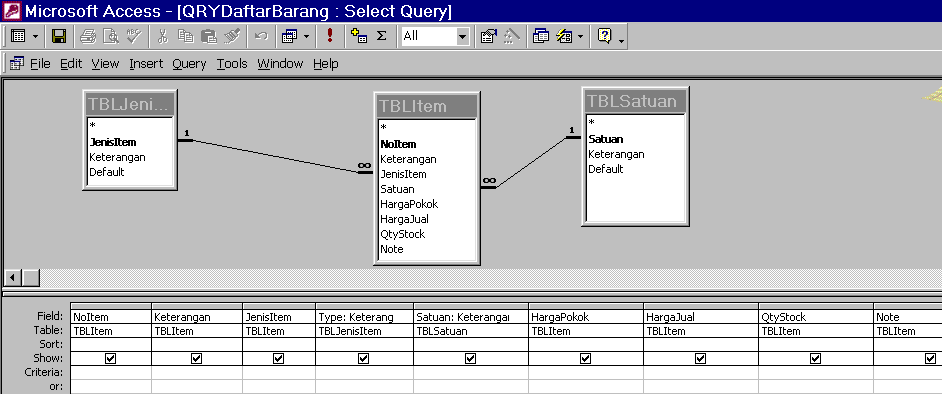
\includegraphics[width=11cm]{gambar_4_2.png}
        \caption{Struktur query DaftarBarang}
        \label{fig:42}
    \end{figure}
    \item Query Laporan Penjualan \newline
    Query ini nantinya dibentuk dari tabel pelanggan, tabel penjualan(header dan detail) serta tabel item. berguna untuk membuat laporan penjualan.
    \begin{figure}[htp]
        \centering
        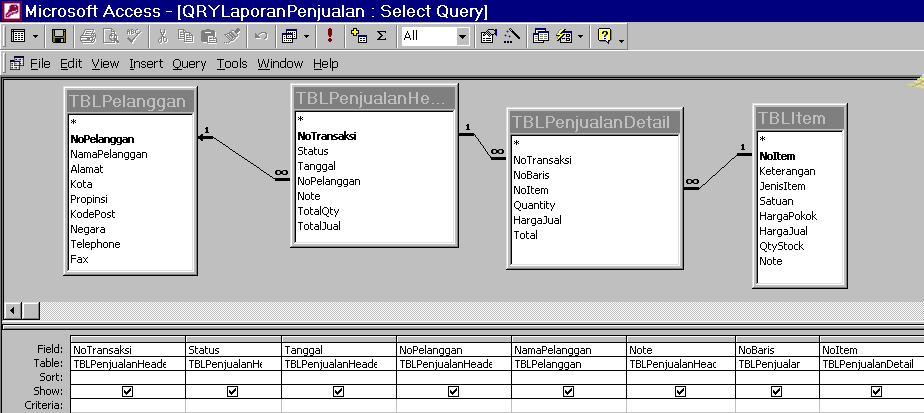
\includegraphics[width=11cm]{gambar_4_3.png}
        \caption{Struktur query laporan penjualan.}
        \label{fig:43}
    \end{figure}
\end{enumerate}

\subsubsection{Implementasi}
Form adalah tempat operator program memasukkan data-data, karena itu desain form dibuat mudah dan lengkap. Form yang terdapat dalam aplikasi ini:
\begin{enumerate}
    \item Form Daftar Barang \newline
    Form ini berfungsi menambah, menghapus, meng-update dan mencari data. Tampilan form daftar barang seperti dibawah
    \begin{figure}[htp]
        \centering
        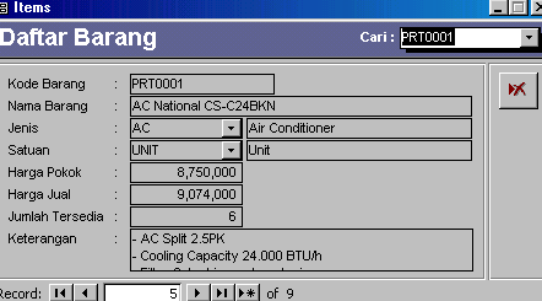
\includegraphics[width=9cm]{gambar_4_4.png}
        \caption{Form daftar barang.}
        \label{fig:44}
    \end{figure}
    \item Form Pelanggan \newline
    Seperti form daftar barang, form ini berfungsi menambah, menghapus, meng-update dan mencari data pelanggan. Tampilan form daftar seperti dibawah
    \begin{figure}[htp]
        \centering
        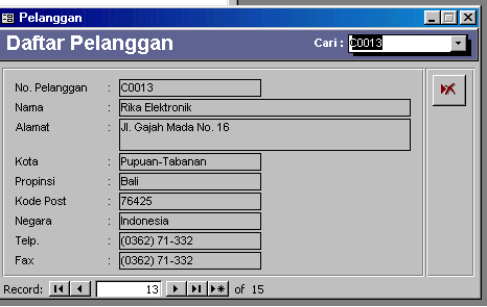
\includegraphics[width=10cm]{gambar_4_5.png}
        \caption{Form Pelanggan.}
        \label{fig:45}
    \end{figure}
    \item Form Penjualan \newline
    Form ini berfungsi mencatat transaksi penjualan dan retur (pengembalian). Operator cukup memilih jenis transaksinya pada combobox status. Pada form penjualan ini terdapat subform penjualandetail. Ini memungkinkan operator untuk mencatat banyak pembelian item barang dalam satu faktur (Nomor Transaksi). Subform ini bentuknya tabular dan bertambah secara otomatis, memungkinkan pencatatan banyak item barang dan total pembelian dihitung secara otomatis pula.
    \begin{figure}[htp]
        \centering
        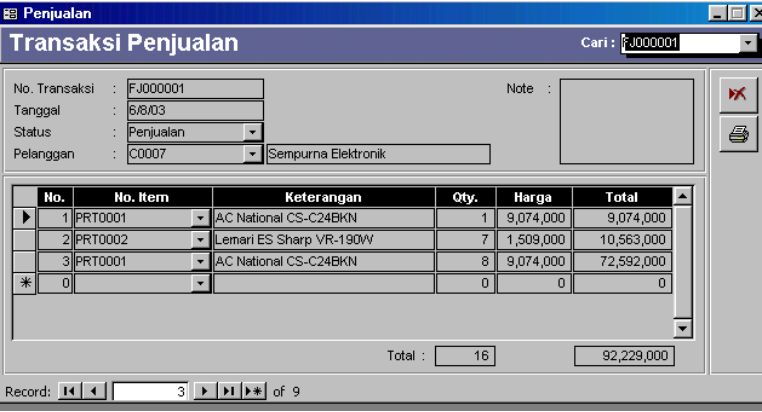
\includegraphics[width=10cm]{gambar_4_6.png}
        \caption{Form penjualan.}
        \label{fig:46}
    \end{figure}
    \item Form keterangan \newline
    Fungsinya untuk menambah satuan dan jenis barang. Form ini juga berfungsi membuat suatu default atau standard satuan dan jenis barang yang digunakan dalam pengisian daftar barang.
    \begin{figure}[htp]
        \centering
        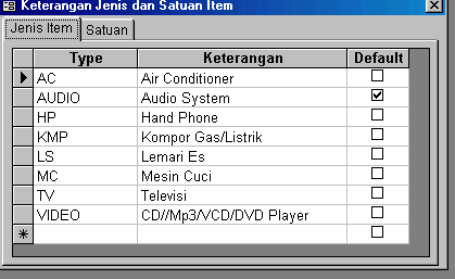
\includegraphics[width=9cm]{gambar_4_7.png}
        \caption{Form keterangan}
        \label{fig:47}
    \end{figure}
    \item Form cetak transaksi \newline
    Fungsinya mencetak transaksi berdaarkan nomor transaksi, pelanggan atau tanggal transaksi. Model tampilan juga dapat dipilih dalam 2 format, yaitu format summary (mencetak jumlah totalnya saja) atau detail (menetak secara lengkap seluruh data transaksi).
    \begin{figure}[htp]
        \centering
        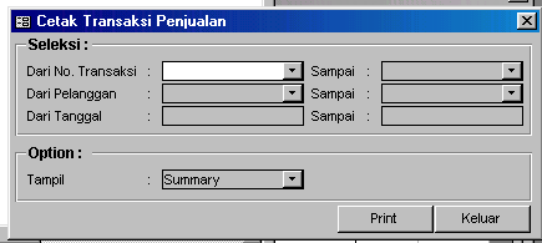
\includegraphics[width=10cm]{gambar_4_8.png}
        \caption{Form cetak transaksi.}
        \label{fig:48}
    \end{figure}
    \item Form menu utama. \newline
    Sebagai form yang pertama tampil (start up). Pada form ini operator program dapat memilih form yang akan ditampilkan. 
    \begin{figure}[htp]
        \centering
        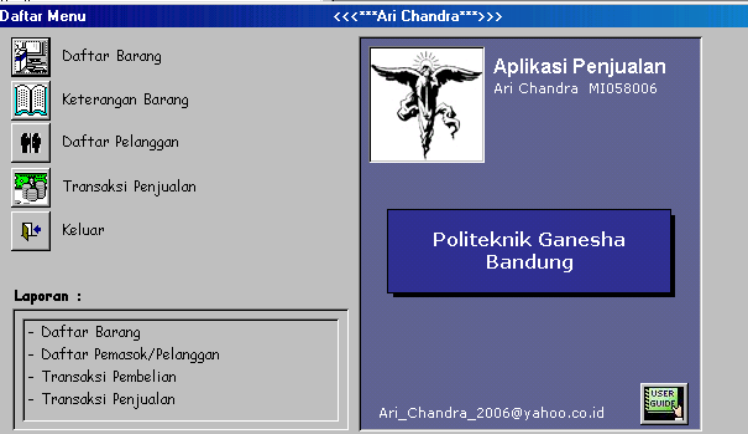
\includegraphics[width=12cm]{gambar_4_9.png}
        \caption{Form menu utama.}
        \label{fig:49}
    \end{figure}
\end{enumerate}

\subsection{Lingkungan Pendukung}
Untuk membangun aplikasi penjualan ini dibutuhkan perangkat keras dan perangkat lunak, yaitu:
\begin{enumerate}
    \item Perangkat Keras
    \begin{enumerate}
        \item Komputer dengan prosesor minimal 166 MHz
        \item Monitor VGA atau dengan resolusi yang lebih tinggi.
        \item Harddisk dengan kapasitas tersedia minimum sebesar kapasitas program.
        \item Keyboard, mouse dan CD ROM.
        \item Printer.
    \end{enumerate}
    \item Perangkat lunak
    \begin{enumerate}
        \item Microsoft Access 2000 atau versi yang  lebih tinggi
        \item Sistem operasi Windows 95/98, atau Windows XP
    \end{enumerate}
\end{enumerate}
Program yang digunakan untuk membangun aplikasi penjualan ini adalah Microsoft Access, karena terdapat banyak fasilitas wizard yang mempercepat pembuatan table, query, form, report.

\subsection{Cara Menggunakan Program}
Karena aplikasi penjualan ini dijalankan pada program Microsoft Access, maka terlegih dahulu kita harus melakukan instalasi Microsoft Office. Langkah langkah instalasinya adalah sebagai berikut
\begin{enumerate}
    \item Masukkan CD Program Microsoft Office ke dalam CD ROM. CD Program Microsoft Office bersifat Auto-run, artinya langsung dijalankan saat windows membaca CD.
    \item Ikuti step-step wizard yang yang ditampilkan. Pastikan pada step Selecting Features, Microsoft Access for Windows dalam keadaan terpilih.
    \newpage
    \begin{figure}[htp]
        \centering
        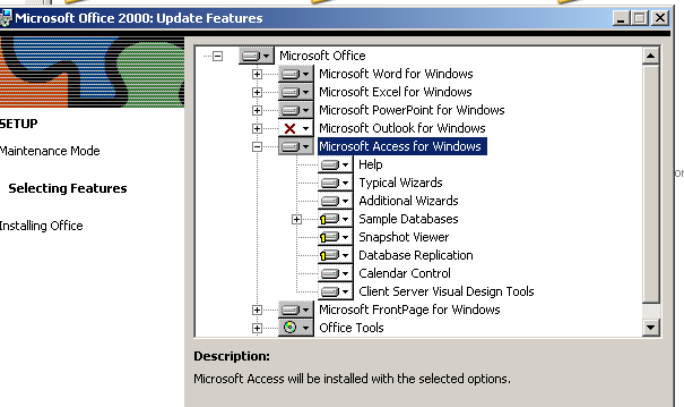
\includegraphics[width=12cm]{gambar_4_10.png}
        \caption{Step Selecting Features pada proses instalasi}
        \label{fig:410}
    \end{figure}
    \item Setelah Microsoft Office dan Microsoft Access terinstal, aplikasi penjualan langsung dikopikan ke harddisk. Agar mempermudah membuka program, dapat dibuat shortcut-nya di desktop. Dengan demikian operator cukup melakukan dobel klik pada shortcut-nya untuk menjalankan program.
    \item Cara menggunakan program ini cukup mudah, operator cukup masuk ke menu daftar barang dan menambahkan data-data item barang yang tersedia.
    \item Untuk menambah data pelanggan, masuk ke menu daftar pelanggan.
    \item Untuk melakukan pencatatan tarnsaksi, masuk ke menu transaksi pembelian, kemudian tentukan status transaksi yang dilakukan (penjualan atau retur).
\end{enumerate}
\section{Kesimpulan}
\subsection{Kesimpulan}
Dari hasil pembuatan perangkat lunak penjualan, kesimpulannya adalah sebagai berikut:
\begin{enumerate}
    \item Aplikasi penjualan dapat mempermudah dan mempercepat pencatatan transaksi penjualan barang.
    \item Biaya pengadaan aplikasi penjualan relatif murah, karena pengoperasiannya tidak membutuhkan komputer dengan spesifikasi tinggi.
    \item Membuat aplikasi penjualan dengan Microsoft Access cukup mudah karena terdapat banyak fasilitas wizard yang mempercepat dan mempermudah pembuatan aplikasi.
\end{enumerate}
\subsection{Saran}
Penulis mengajukan beberapa saran yang mungkin dapat dipertimbangkan, yaitu:
\begin{enumerate}
    \item Mengingat pentingnya pencatatan transaksi yang akurat, maka proses tersebut lebih baik dilakukan secara terkomputerisasi dan aplikasi penjualan ini merupakan solusi yang baik untuk permasalahan tersebut.
    \item Aplikasi penjualan dibuat dengan tampilan user friendly, mudah digunakan. Tetapi lebih baik operator program harus memiliki pengetahuan dasar tentang sistem operasi Windows.
\end{enumerate}
\newpage
\section*{Daftar Pustaka}

Budiman, H.A. 2004. Internet dan Web Server, Yogyakarta :   Penerbit Andi \newline \newline
Lubis, Adnan, 1981. Prosedur dan Metode Penyusunan Sistem Akuntansi, Jakarta: Pustaka Amani \newline \newline
Maulana, Edwin, 2002. Aplikasi Microsoft Access untuk Inventory, Jakarta : Madcoms.

    
\end{document}
